\documentclass[apectratio=169]{beamer}
\usetheme{metropolis}           % Use metropolis theme
% For PDFs
\newcommand{\myast}{\ensuremath{^{\ast}}}
\newcommand{\mydagger}{\ensuremath{^{\dagger}}}
\usepackage[utf8x]{inputenc}
\usepackage{pdfpages}
\usepackage{minted}
\usepackage{siunitx}
\title{Enabling Ambient Backscatter\\
Using a Low-Cost Software Defined Radio}
\subtitle{Saving Energy/Low Power Communications}
\date{\vspace{1em}
\today}
\author{Maximilian Stiefel\myast, Elmar van Rijnswou\myast\\Carlos Pérez-Penichet\myast, Ambuj Varshney\myast, Christian Rohner\myast and Thiemo Voigt \mydagger
\vspace{1em}
\\\myast Uppsala University
\\\mydagger Uppsala University and RISE SICS
}
\institute{13th Swedish National Computer Networking Workshop}
\begin{document}
  \maketitle

\begin{frame}{Contributions}
	\begin{itemize}
		\item<1-> First system using the RTL-SDR to receive ambient backscatter
		\item<2-> Showing that ambient backscatter using TV signals to be feasible in wider parts of the city \only<3->{\ensuremath{\rightarrow} Significant improvement of the state-of-the-art, which is restricted to a TV towers proximity}
	\end{itemize}
\end{frame}

\section{Introduction}

\begin{frame}{What is Backscattering? (1)}
	\begin{figure}[H]	
		\centering
		\only<1>{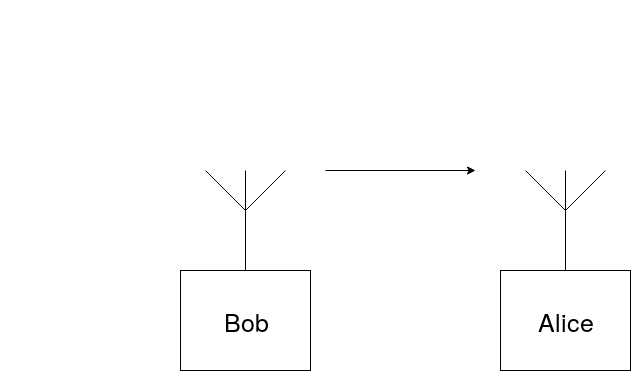
\includegraphics[width=0.7\textwidth]{./fig/backscatter_simpler}}
		\only<2->{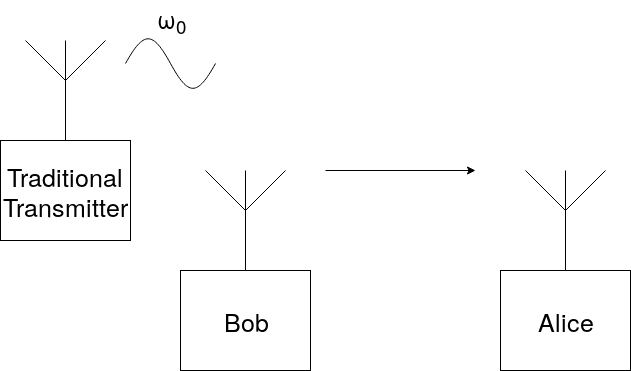
\includegraphics[width=0.7\textwidth]{./fig/backscatter_simple}}

		\caption{Simplest form of backscattering. Simplex with two subscribers.}
	\end{figure}
	\metroset{block=fill}
	\only<3>{\begin{block}{Backscattering}
		Communication technique similar to passive RFID, but the transmitter has to maintain its signal. 
	\end{block}}
\end{frame}

\begin{frame}{What is Backscattering? (2)}
\begin{minipage}{0.45\textwidth}
	\begin{figure}[H]	
		\centering
		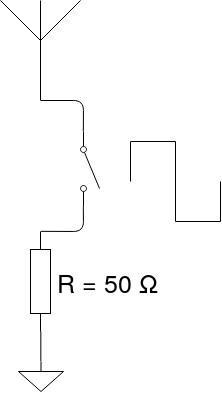
\includegraphics[height=0.5\textheight]{./fig/rfswitch}
		\caption{\SI{50}{\ohm} connected to a RF switch do the trick.}
	\end{figure}
\end{minipage}
\hfill
\begin{minipage}{0.45\textwidth}
	\only<2->{\begin{equation}
		P_R = P_A \cdot (1-\Gamma^2)
	\end{equation}}
	\only<3->{\begin{equation}
		\Gamma = \frac{Z_L - Z_A}{Z_L + Z_A}
	\end{equation}}
	\only<4->{Total reflection: 
	\begin{equation*}
		\lim_{Z_L \to \infty} \Gamma = \frac{Z_L - Z_A}{Z_L + Z_A} = 1
	\end{equation*}}
	\only<5->{Total absorption: 
	\begin{equation*}
		\lim_{Z_L \to \SI{50}{\ohm}} \Gamma = \frac{Z_L - Z_A}{Z_L + Z_A} = 0
	\end{equation*}}
\end{minipage}
\end{frame}

\begin{frame}{Frequency Shift Keying With Backscatter Tags (1)}
	\begin{figure}[H]	
		\centering
		\only<1>{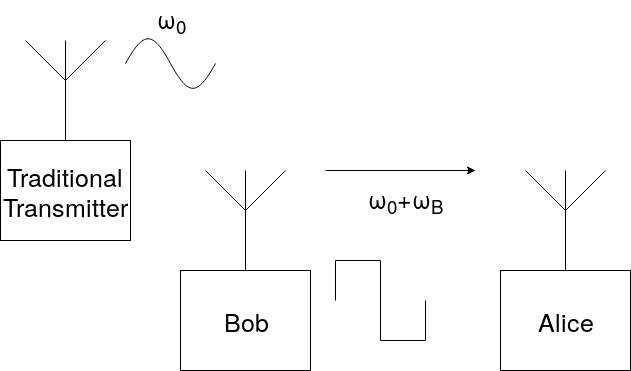
\includegraphics[width=0.8\textwidth]{./fig/backscatter}}
		\caption{Frequency shift keying modulation techniques are enabled by switching with a higher frequency.}
	\end{figure}
	\metroset{block=fill}
\end{frame}

\begin{frame}{Frequency Shift Keying With Backscatter Tags (2)}
	\only<1->{\begin{figure}[H]	
		\centering
		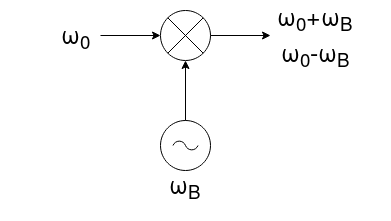
\includegraphics[width=0.5\textwidth]{./fig/mixer}
		\caption{Classical communications engineering element: The mixer.}
	\end{figure}}
	\only<2->{\begin{equation}
	2\sin(\omega_0 t) \sin(\omega_B) = \cos[(\omega_0 + \omega_B)t] - \cos[(\omega_0 - \omega_B) t]
	\label{eq:mixing}
	\end{equation}}

\end{frame}

\begin{frame}{Why Backscattering?}
	\begin{itemize}
		\item<1-> Ultra-low power wireless transmissions by reflecting/absorbing EM waves (in orders of \SI{}{\micro\watt}) \cite{liu_ambient_2013}
		\item<2-> Leverage existing signals such as coming from WiFi \cite{hitchhike,kellogg2015wi} or TV towers \cite{liu_ambient_2013,parks_turbocharging_2014}
		\item<3-> Mechanism of choice to network devices operating on harvested energy
		\item<4-> Communication frontends much simpler, smaller and cheaper, in comp. with traditional RF frontends
	\end{itemize}
\end{frame}

\begin{frame}{TV Signal Backscattering Application Example}
\begin{minipage}{0.45\textwidth}
	\begin{figure}[H]	
		\centering
		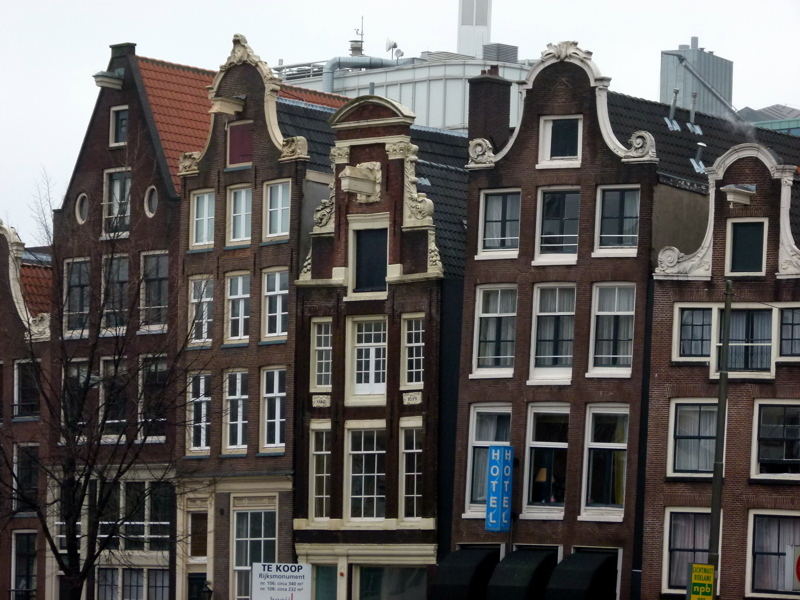
\includegraphics[height=0.5\textheight]{./fig/elmars_home}
		\caption{Houses in Amsterdam. Source: reddit.com}
	\end{figure}
\end{minipage}
\hfill
\begin{minipage}{0.45\textwidth}
	\begin{itemize}
		\item<1-> Houses in the Netherlands are constantly sinking
		\item<2-> Backscattering tags on the roofs next to the TV antenna
		\item<3-> Sensor network with node which are highly-energy constrained
	\end{itemize}
\end{minipage}
\end{frame}


\section{Looking for TV Signals in Uppsala}

\begin{frame}{Spatial Variation of Ambient TV Signals (1)}
\begin{figure}[h]
	\centering
	\begin{minipage}{0.49\columnwidth}
		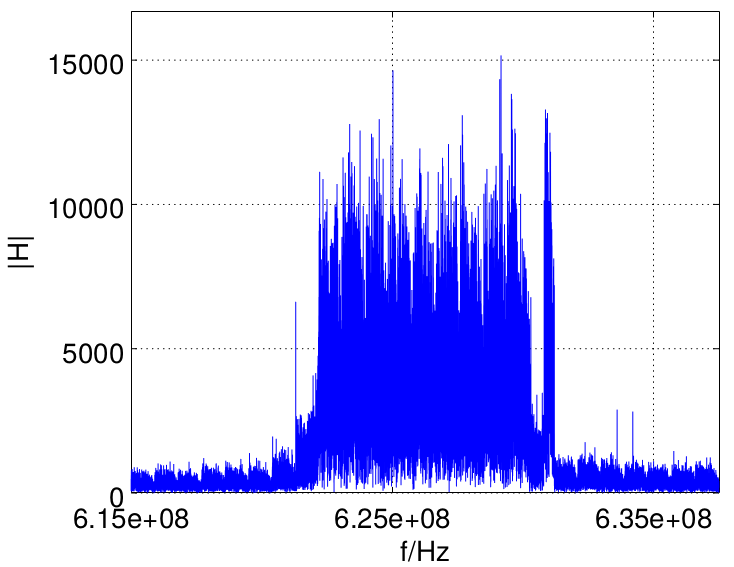
\includegraphics[width=\columnwidth]{./fig/626mhz_raw}
	\end{minipage}
	\hfill
	\begin{minipage}{0.49\columnwidth}
		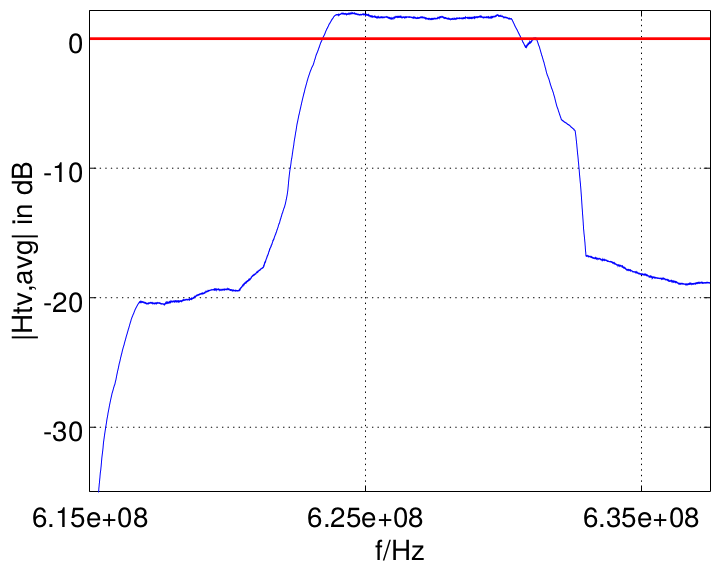
\includegraphics[width=\columnwidth]{./fig/626mhz_filtered}
	\end{minipage}
	\caption{Single measurement at one point in space. Left: Raw spectrum. Right: Spectrum where average power had been determined.}
	\label{fig:tv_record} 
	\end{figure}
\end{frame}

\begin{frame}{Spatial Variation of Ambient TV Signals (2)}
\begin{figure}[h]
	\centering
	\begin{minipage}{0.49\columnwidth}
		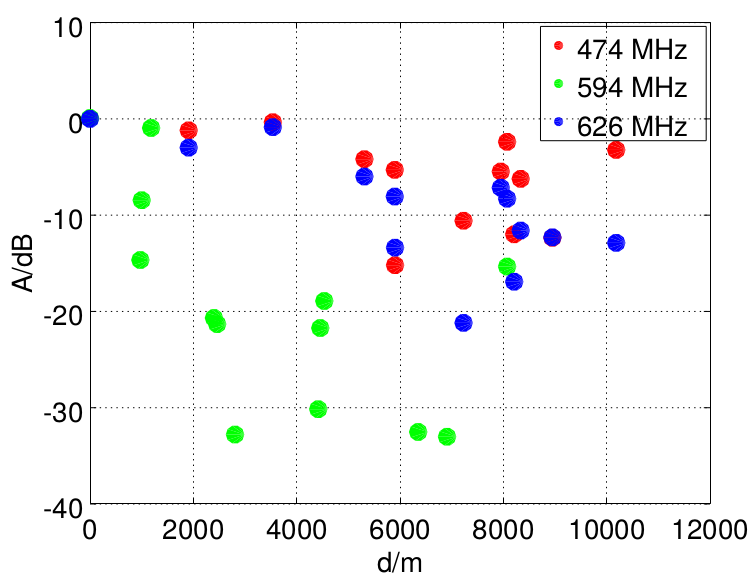
\includegraphics[width=\columnwidth]{./fig/haversine}
	\end{minipage}
	\hfill
	\begin{minipage}{0.49\columnwidth}
		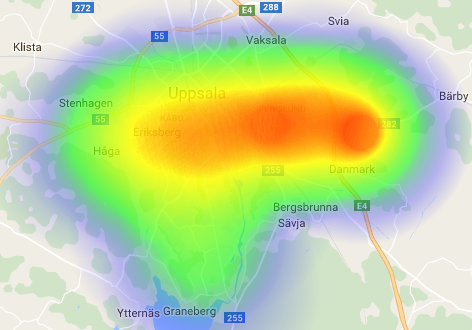
\includegraphics[width=\columnwidth]{./fig/heatmap_626mhz}
	\end{minipage}
	\caption{Multiple measuremnets in space. Left: Signal attenuation vs. distance from TV tower. Right: Interpolated heatmap for the \SI{626}{\mega\Hz}.}
	\label{fig:haversine}
\end{figure}
\end{frame}


\begin{frame}{Backscattering a Local Signal}
	\begin{figure}[H]	
		\centering
		\only<1>{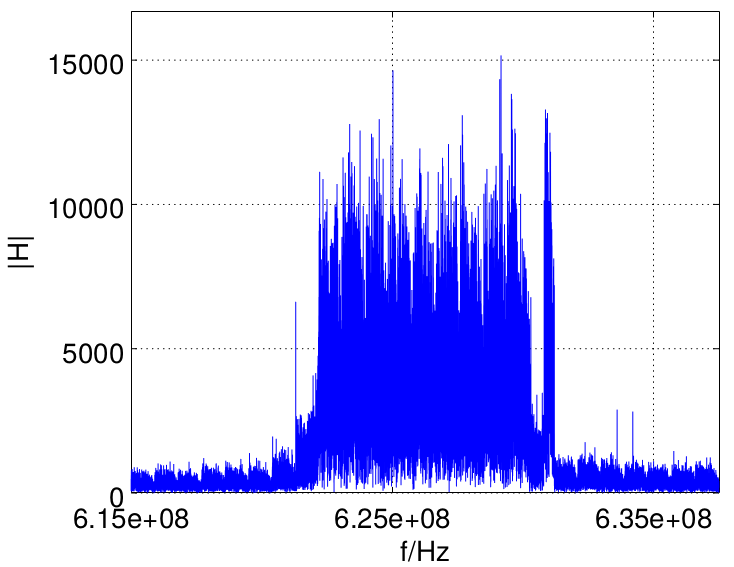
\includegraphics[width=0.7\textwidth]{./fig/626mhz_raw.png}}
			\only<2>{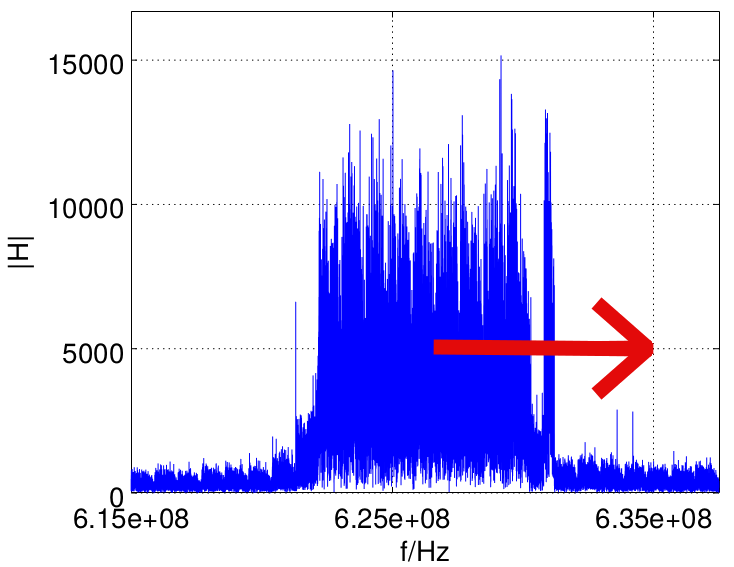
\includegraphics[width=0.7\textwidth]{./fig/626mhz_raw_arrow.png}}	
		\caption{Spectrum of a local TV signal. Center frequency is \SI{626}{\mega\Hz}.}
	\end{figure}	
\end{frame}

\section{Communication System Design}

\begin{frame}{Transmitter (1)}
	\only<1>{\begin{figure}[H]	
		\centering
		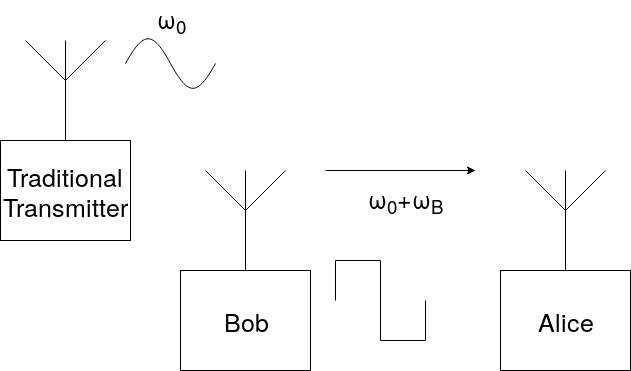
\includegraphics[width=0.7\textwidth]{./fig/backscatter}
	\end{figure}}
	
	\only<2>{\begin{figure}[H]	
		\centering
		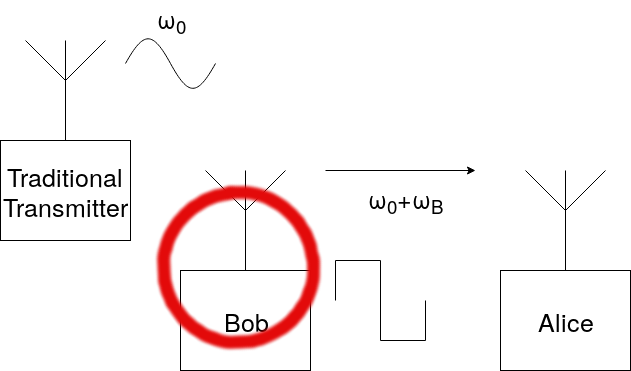
\includegraphics[width=0.7\textwidth]{./fig/backscatter_simple_bob}
	\end{figure}}
\end{frame}

\begin{frame}{Transmitter (2)}
	\begin{figure}[H]	
		\centering
		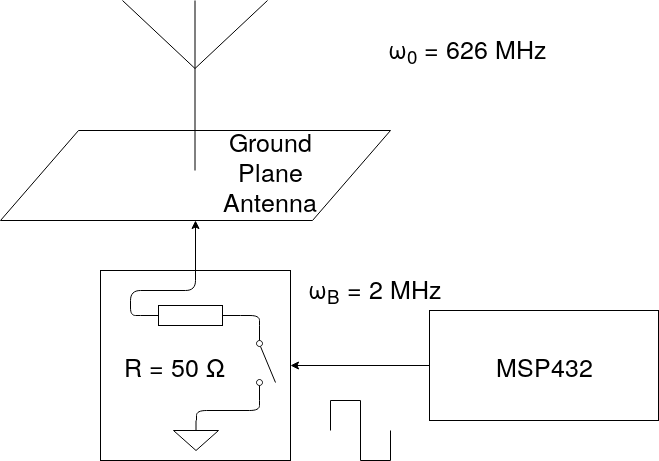
\includegraphics[width=0.7\textwidth]{./fig/transmitter}
		\caption{Transmitter architecture. Ground plane antenna roughly tuned to TV signal center freq. (\SI{626}{\mega\Hz}). Microcontroller steers a RF switch with a rectangular signal shifting the TV wave in another band.}
	\end{figure}
\end{frame}

\begin{frame}{Receiver (1)}	
	\only<1>{\begin{figure}[H]	
		\centering
		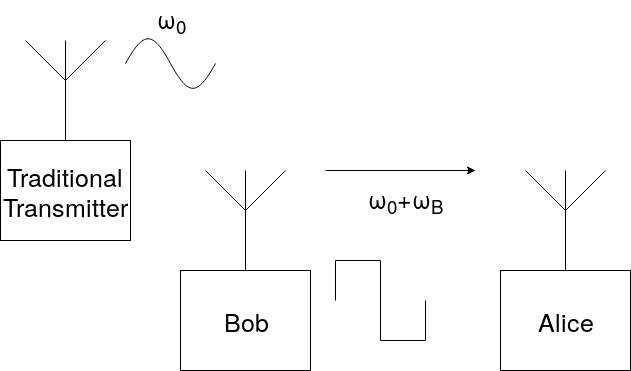
\includegraphics[width=0.7\textwidth]{./fig/backscatter}
	\end{figure}}
	
	\only<2>{\begin{figure}[H]	
		\centering
		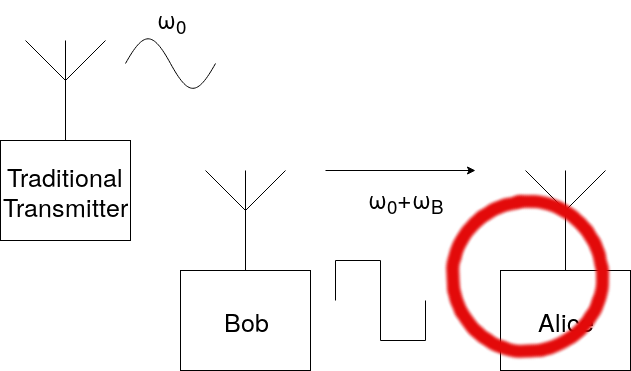
\includegraphics[width=0.7\textwidth]{./fig/backscatter_simple_alice}
	\end{figure}}
\end{frame}

\begin{frame}{Receiver (2)}

\begin{minipage}{0.45\textwidth}
	\begin{figure}[H]	
		\centering
		\only<1>{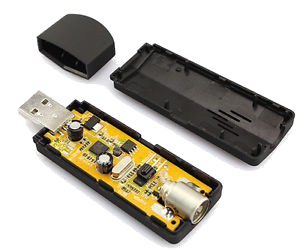
\includegraphics[width=0.8\textwidth]{./fig/rtlsdr}}
		\only<2,3>{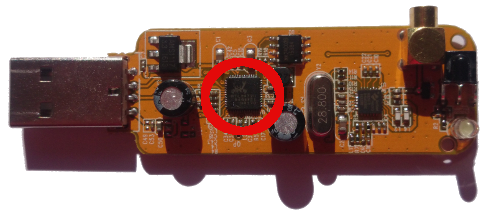
\includegraphics[width=0.8\textwidth]{./fig/rtlsdr1}}
		\only<4>{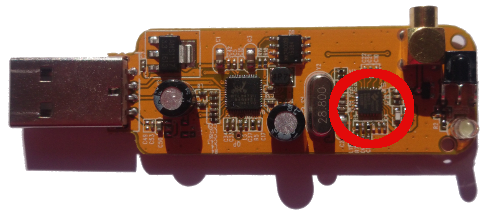
\includegraphics[width=0.8\textwidth]{./fig/rtlsdr2}}
		\caption{RTL-SDR hardware with the DVB-T I/Q demodulator
		Raeltek RTL2832U (left IC) and the tuner with integrated LNA
		Rafael Micro R820T/2 (right IC).}
	\end{figure}
\end{minipage}
\hfill
\begin{minipage}{0.45\textwidth}
	\begin{itemize}
		\item<2-> RTL2832U is cheap  
		\item<3-> Access to I/Q demodulator (DAB and FM radio) can be hacked		\item<4-> Tuner (LNA, filters etc.) included
	\end{itemize}
\end{minipage}
\end{frame}

\begin{frame}{Receiver (3)}
	\begin{figure}[H]	
		\centering
		\only<1>{
\includegraphics[width=0.9\textwidth]{./fig/receiver1}}
		\only<2>{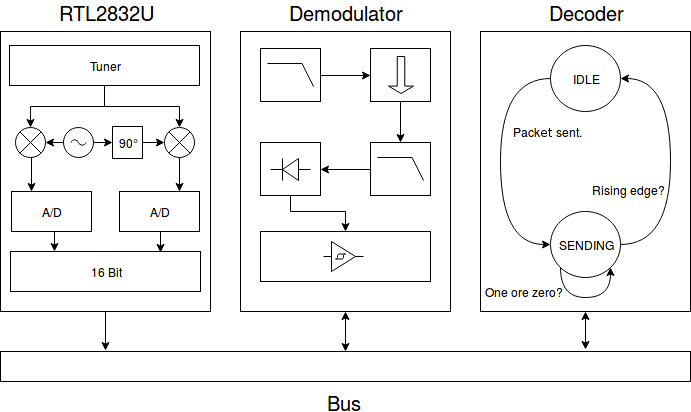
\includegraphics[width=0.9\textwidth]{./fig/receiver2}}
		\caption{Architecture of backscatter receiver.}
	\end{figure}
\end{frame}

\section{Results and Outlook}

\begin{frame}{Communication Performance (1)}
	\begin{figure}[h]
	\centering
	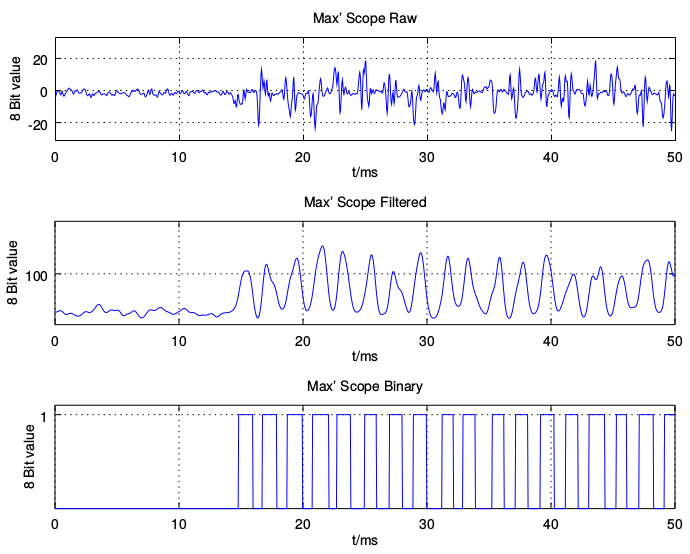
\includegraphics[width=0.7\textwidth]{./fig/transmission}
	\caption{Start of a transmission. Different signal processing steps are visible. First: Raw downsampled signal amplitude. Second: Signal after low-pass filter. Third: Signal after Schmitt trigger.}
	\label{fig:transmission}	
\end{figure}
\end{frame}

\begin{frame}{Communication Performance (2)}
	\begin{itemize}
		\item<1-> We varied the bitrate between 1 bit/s and 1 kbit/s 
		\item<2-> Strength of the backscattered signal is quite low (high quantisation noise)
		\item<3-> Higher bitrates (1 kbit/s) lead to a range of a couple of decimeter before the error rate goes up rapidly
		\item<4-> High bit error rate is due to the not yet customized HW
	\end{itemize}
\end{frame}

\begin{frame}{Results}
	\begin{itemize}
		\item<1-> Spectrum scanning over a huge band is possible using the RTL-SDR
		\item<2-> Uppsala is adequate for backscatter communication using our receiver
		\item<3-> Backscatter communication is possible with the RTL-SDR
	\end{itemize}
\end{frame}

\begin{frame}{Outlook}
	\begin{itemize}
		\item<1-> Other antennas for reception and transmission have to be tried out
		\item<2-> Standard cable and antenna of the RTL-SDR (included in the 10 USD budget) are unsuiteable for our application as we realized
		\item<3-> The filters involved are setscrews as well as the coding used by the communication system
	\end{itemize}
\end{frame}



\begin{frame}[standout]
	Thank you for your attention. 
\end{frame}

\begin{frame}[allowframebreaks]{References}

  \bibliography{presentation}
  \bibliographystyle{apalike}

\end{frame}

\end{document}
